\documentclass[12pt,twoside]{article}
\usepackage[dvipsnames]{xcolor}
\usepackage{tikz,graphicx,amsmath,amsfonts,amscd,amssymb,bm,cite,epsfig,epsf,url}
\usepackage[hang,flushmargin]{footmisc}
\usepackage[colorlinks=true,urlcolor=blue,citecolor=blue]{hyperref}
\usepackage{amsthm,multirow,wasysym,appendix}
\usepackage{array,subcaption} 
% \usepackage[small,bf]{caption}
\usepackage{bbm}
\usepackage{pgfplots}
\usetikzlibrary{spy}

\pgfplotsset{compat=1.18}
\usepackage{thmtools}
\usepackage{blkarray} 
\usepackage{textcomp}
\usepackage[left=0.8in,right=1.0in,top=1.0in,bottom=1.0in]{geometry}
\newcommand{\Lagr}{\mathcal{L}}
\newcommand{\Id}{Id}
\newcommand{\R}{\mathbb{R}}

\begin{document}

\section*{1014 Linear Algebra - Final Notes}

\section*{Norms}
\textbf{Definition of Norms}:
\begin{enumerate}
    \item Homogeneity: $||\alpha v|| = |\alpha| \times ||v||$ for all $\alpha \in \R^n$ and $v \in V$
    \item Positive Definiteness: if $||v|| = 0$ for some $v\in V$ then $v=0$
    \item Triangular Inequality: $||u+v|| \leq ||u|| + ||v|| $ for all $u,v \in V$
\end{enumerate}
\section*{Inner Products} 
\textbf{Definition of Inner Products} 
\begin{enumerate}
    \item Symmetry: $\langle u, v \rangle = \langle v, u \rangle$ for all $u,v \in V$
    \item Linearity: $\langle u+v, w \rangle = \langle u,w\rangle + \langle v,w\rangle$ and $\langle \alpha v , w\rangle = \alpha \langle v,w\rangle$ for all $v,u,w \in V$ and $\alpha \in \R$
    \item Positive Definiteness: $\langle v,v \rangle \geq 0$ with equality if and only if $v=0$
\end{enumerate}
\textbf{Proposition}:
If $\langle \cdot,\cdot \rangle $ is an inner product on $V$ then $$
    ||v|| = \sqrt{\langle v,v \rangle}
$$ is a norm on $V$. We say that the norm $||\cdot|| $ is induced by the inner product $\langle \cdot, \cdot \rangle$\\
\textbf{L1 Norm}\\
The Euclidean Norm is the sum of the absolute values $i^{th}$ entry in the input vector.
$$
    ||x||_1 = \sum_{i=1}^n |x_i|
$$
\textbf{Euclidean Norm:}\\
The Euclidean Norm is the square root of the sum of the products of each $i^{th}$ entry in the input vectors.
$$
    ||x||_2 = \sqrt{\langle x, x \rangle } = \sqrt{x_1^2 + \dots + x_n^2}
$$
\textbf{Cauchy-Schwartz Inequality}
Let $||\cdot||$ be the norm induced by the inner product $\langle \cdot, \cdot \rangle$ on the vector space $V$. Then for all $x,y \in V$:
$$
    |\langle x,y \rangle|  \leq ||x|| \times ||y||
    $$
Moreover, there is equality if and only if $x$ and $y$ are linearly dependent (i.e. $x=\alpha y$ or $y= \alpha x$ for some $\alpha \in \R)$

\section*{Orthogonality}
\textbf{Definition of Orthogonality}:
Let $V$ be a vector space and $\langle \cdot, \cdot \rangle$ be an inner product on $V$
\begin{itemize}
    \item We say that vectors $x,y$ are orthogonal  if $\langle x,y \rangle = 0$. We write $x \perp y$
    \item We say that vector $x$ is orthogonal to the set of vectors $A$ if $x$ is orthogonal to all of the vectors in $A$. We write $x \perp A$
\end{itemize}
\textbf{Orthonormal Family of Vectors:}\\
For a Orthonormal Family of Vectors $\{v_1,\dots, v_n \}$
\begin{itemize}
    \item The family is orthogonal if $\langle v_i, v_j \rangle =0$ for all $i \neq j$
    \item The family is orthonormal if all the vectors are orthogonal and all of the $v_i$ have unit norm $||v_1|| = \dots = ||v_k|| = 1$
    \item Orthonormal basis preserve distance and angles: $\langle Ax, Ay\rangle = x^TA^TAy = x^Ty = \langle x,y \rangle$
    \item A vector space of finite dimension admits an orthonormal basis
    \item Assume that $dim(V)=n$ and let $v_1, \dots, v_n$ be an orthonormal basis of $V$. Then the coordinates of a vector $x \in V$ in the basis $v_1, \dots, v_n$ are
$$
    x = \langle x, v_1 \rangle v_1 + \dots + \langle x,v_n \rangle v_n 
$$
\end{itemize}
\textbf{Pythagorean Theorem:}\\
Let $||\cdot||$ be the norm induced by $\langle \cdot, \cdot \rangle $ for all $x,y \in V$ we have:
$$
    x \perp y \longleftrightarrow ||x+y||^2 = ||x||^2 + ||y||^2
$$
\textbf{Proof of Pythagorean Theorem:}
\begin{equation}
    \begin{split}
        ||x+y||^2 &= \langle x+y , x+y \rangle  \\
        &= \langle x , x \rangle + \langle y , y \rangle + 2\langle x , y \rangle \\
        &= ||x||^2 + ||y||^2 \text{ as } x \perp y \text{ so } \langle x,y \rangle = 0 \qed
    \end{split}
\end{equation}
\textbf{Orthogonal Projection}
Let $S$ be a subspace of $R^n$ The orthogonal projection of a vector $x$ onto $S$ is defined as the vector $P_S(x)$ in $S$ that minimizes the distance to $x$:
$$
    P_S(x) = argmin ||x-y|| \ \ for \ y\in S
$$
The distance from $x$ to the subspace $S$ is defined by:
$$
    d(x,S) = min||x-y|| = ||x-P_S(x)|| 
$$
\textbf{Projection Matrix:} $VV^Tx$
\textbf{Projection Formula:} $P_S(x) = \langle v_i, x \rangle v_i + \dots + \langle v_n, x \rangle v_n$
\section*{Eigenvectors, Square Symmetric Matrices, and SVD}
\textbf{Properties of Eigenvectors:}
\begin{enumerate}
    \item If $v_i$ is an eigenvector with associated eigenvalue $\lambda_i$, then: $Av_i = \lambda_i v_i$
    \item If you scale a matrix $A$ by some constant $\alpha \in \R$, its eigenvalues get shifted by $\alpha$ as: $\alpha Av_1 = \alpha \lambda_i v_i$ where $v_i$ is an eigenvalue of A.
    \item Likewise, if you add to the diagonals of a matrix $A$ using the identity to a matrix, the eigenvalues of $A$ get scaled by $\alpha$: $(A+\alpha \times Id_n)v_i = \alpha v_i + Av_i = \alpha v_i + \lambda_i v_i = v_i(\alpha + \lambda_i)$
    \item If you have two eigenvectors, that share the same eigenspace and eigenvalue, any linear combination is also a eigenvector in that eigenspace with that eigenvalue:
    $$
        Av_1 = \lambda_1 v_1 \text{ and } Av_2 = \lambda_1 v_2 \text{ then } A(v_1 + v_2) = A(v_1) + A(v_2) = \lambda_1 v_1 + \lambda_1 v_2 = \lambda_1(v_1+v_2) \qed
    $$ Note: that this does not hold if the two eigenvectors do not share the same eigenspace (and therefore, eigenvalue).
    \item If you are given a eigenvalue, $\lambda$ to solve for the eigenspace and thus eigenvector(s) associated with the eigenvalue, you do: $Ker(A-(\lambda \times \Id_n))x=0$ and solve for x via row reduction.
\end{enumerate}
\textbf{Square Symmetric Matrices:}
\begin{enumerate}
    \item Any square, symmetric matrix $S$ Can be expressed as $S = PDP^T$, where $P$ is the orthonormal eigenvector basis of S. If S is PSD then its eigenvalue are PSD 
    \item This be interpreted geometrically as a rotation, then a scaling, then a rotation back to canonical coordinates
    \item If there is a kernel, the matrix is not invertible, and at least one eigenvector will be associated to the eigenvalue equal to 0
    \item The sum of its eigenvalues is equal to its trace $Tr(A) = Tr(PDP^T) = Tr(P^TPD) = Tr(D)$
\end{enumerate}
\textbf{PCA} When doing PCA we pick the largest eigenvalue, as it maximizes the variance. If you take a vector, x where $x=\alpha_1v_1 + \dots + \alpha_n v_n$ and $||x|| = 1$, where $v_1, \dots, v_n$ are eigenvalues of some orthonormal eigenbasis. We then maximize $x^TAx$ \\ 
\textbf{Trace} $Tr(AB) = Tr(CB)$ then $Tr(A) = \sum_{i=1}^n \lambda_i$ where $A \in \R^{n \times n}$ and $A$ is square symmetric.
\section*{SVD: Singular Value Decomposition:}
Any matrix $A \in \R^{n\times m}$ (any matrix though even if the dimensions match) can be written in its SVD form as: $A = U\Sigma V^T$ where $\Sigma \in \R^{n \times m}$ is a diagonal matrix with the singular values in the diagonal and 0's everywhere else, $V = Eig(A^TA), \ and \ V \in \R^{m\times m}$ and $U = Eig(AA^T), \ and \ U \in \R^{n \times n}$, where $Eig()$ indicates an orthonormal basis of eigenvectors belonging to some matrix. Some useful identities:
$$
    A = U \Sigma V^T \qquad  A^TA = V\Sigma^T \Sigma V^T = V\Sigma^2 V^T \qquad AA^T = U \Sigma V^T V \Sigma U^T = U \Sigma^2 U^T
$$
The Moore-Penrose psuedo-inverse is defined as:
$$
    A^\dagger = V\Sigma^\prime U^T \qquad \text{where } \Sigma^\prime \text{ is a diag matrix of }
$$
\section*{Convexity}
\textbf{Convex Sets:}\\
A set, $M$ is convex if its elements satisfy the following property: that 
$$\alpha x + (1-\alpha) y \in M \text{ for } \alpha \in [0,1] \text{ and } x,y \in M$$ 
\textbf{Convex Functions:}\\
A function is said to be convex if any line drawn from two points in the function rests above the actual value of the function at that point. Expressed mathematically by:
$$
    f(\alpha x + (1-\alpha)y) \leq \alpha f(x) + (1-\alpha)f(y) \text{ with } \alpha \in [0,1]
$$
A function is strictly convex if there is strict inequality, which means there is only one minimum point of the function.\\
\textbf{Properties of Convexity:}
\begin{enumerate}
    \item A function $f$ is called concave if $-f$ is convex
    \item Any linear map is convex and concave: $f(\alpha x + (1-\alpha)y) = \alpha f(x) + (1-\alpha)f(y) \text{ with } \alpha \in [0,1]$. Also, any norm is convex and the gradient is orthogonal to contour lines.
    \item The sum of two convex functions is also a convex function. \textbf{If there is a scalar $\alpha$ multiplying one of the two functions, then this does not hold}
    \item The graph of a convex function will always be above (or equal) to its tangent $$
        f(y) \geq f(x) + \langle \nabla f(x), (y-x)\rangle 
    $$
    \item The Hessian is Square Symmetric, and you can tell if the Hessian, and thus function, is PSD/PD/ND/NSD by looking at the eigenvalues.
    \item $f$ is only convex if and only if for all $x\in \R^n$ $H_f(x)$ is PSD . If the Hessian is PD then its strictly convex. Likewise if the Hessian is NSD its concave, and ND then strictly concave. Note that if there are variables in the Hessian, you know its not a convex function, though it could be convex in certain ranges. 
    \item $A^TA$ and $AA^T$ are always PSD, and if $A$ is full rank, then $A^TA$ is PD. Therefore, it's Hessian will be strongly/strictly convex.
    \end{enumerate}
\textbf{Taylor's Formulas:}
$$
    Order \ 1 \rightarrow f(x+h) = f(x) + hf^\prime(x) \qquad  Order \ 2 \rightarrow f(x+h) = f(x) + h\nabla f(x) + \frac{h^2}{2}f^{\prime \prime}(x)
$$
\textbf{Linear Algebra Form:} 
$$
    Order \ 1 \rightarrow f(x+h) = f(x) + \langle h, \nabla f(x) \rangle \qquad  Order \ 2 \rightarrow f(x+h) = f(x) + \langle h, \nabla f(x) \rangle + \frac{1}{2}h^TH_f(x)h
$$
    
\section*{Regression}
\textbf{Ordinary Least Squares}
\begin{enumerate}
    \item We want to solve the problem $Ax=b$, but unfortunately, unless our matrix is square and full rank there won't be a solution. A tall matrix risks not having y in its image, and a fat matrix will have a null space, thus there will be infinitely many solutions.
    \item We define the problem as Minimize $f(x) = ||Ax-y||^2 = \langle Ax-y, Ax-y \rangle$ with respect to $x\in \R^d$. If the matrix has no kernel, the set of solutions is given by: $x = (A^TA)^{-1}A^Ty$
    \item If $A^TA$ is not invertible, which means that A is not full rank and admits a kernel, as $Ker(A^TA) = Ker(A)$, then we will have to use the MP psuedo-inverse, defined as $A^\dagger = V\Sigma^\prime U^T$, then $x^{LS} = A^\dagger y$ and it is a solution to $A^TAx = A^Ty$
    \begin{equation}
        \begin{split}
            A^Ty &= A^\dagger y \\
            A^TAx &= V\Sigma^\prime U^T y \\
            x &= (A^TA)^{-1} (V\Sigma^\prime U^T y)\\
            x &= (V\Sigma^TU^TU\Sigma V^T)(V\Sigma^\prime U^T y) \\ 
            x &= V\Sigma U^Ty = A^T y \qed
        \end{split}
    \end{equation}
    \item Again, but more detail identities:
    \begin{equation}
        \begin{split}
            (A^TA)^{-1}A^Ty =& (V\Sigma^T U^T U \Sigma V^T)^{-1}A^Ty \\
            =& V\Sigma^{-2}V^T(A^Ty) \\
            =& V\Sigma^{-2}V^T(V\Sigma^TU^Ty) = V\Sigma^\prime U^Ty \\
            =& A^\dagger y
        \end{split}
    \end{equation}
    \item If there is a kernel, the set of all minimizers is given by $\{ x^{LS} + v | v \in Ker(A) \}$
\end{enumerate}
\textbf{Ridge Regression}
\begin{enumerate}
    \item We define the problem as Minimize $f(x) = ||Ax-y||^2 + \lambda ||x||_2^2$ w.r.t. $x\in \R^d$
    $$
    x^{ridge} = (A^TA + \lambda Id_n)A^Ty
    $$
    \item Implies $f(x)$ is a strongly convex function, and therefore strictly convex.
\end{enumerate}
\textbf{LASSO Regression}
\begin{enumerate}
    \item We define Lasso regression as adding the L1 norm as a penalty to the least squares problem: $f(x) = ||Ax-y||^2 + \lambda ||x||_1$
\end{enumerate}
    
\section*{Matrix Norms}
\textbf{NOTE: NORMS (BOTH MATRIX AND VECTOR) ARE NOT LINEAR MAPS!} i.e. $||-x||_2 \neq -||x||_2$ \\
\textbf{Frobenius Norm:} a norm on a matrix $A \in \R^{n \times m}$ is defined as $$
        ||A||_F = \sqrt{\sum_{i=n}^n \sum_{j=1}^m A_{i,j}^2} = Tr(A^TA) = \sqrt{\sum_{i=1}^{min(n,m)} \sigma_i (A)^2}
$$
Proof: $||A||_F^2 = Tr(AA^T) = Tr( U\Sigma V^T V \Sigma^T U) = Tr(\Sigma \Sigma ^T) = \sum_{i=1}^{min(n,m)} \sigma_i (A)^2$ \\ 
\textbf{Spectral Norm:} $||A||_{sp} = \arg max_{||x||=1} ||Ax|| = \sigma_1 (A) $ \\
\textbf{Nuclear Norm:} L1 Norm for matrices $||A||_* = \sum_{i=1}^{min(n,m)} \sigma_i (A)$
\section*{Optimality Conditions:}
Isotropic $->$ eig vals are in really close ratio\\
Anistropic they are not
\section*{Constrained Optimization}
\textbf{Lagrangian Functions}
\begin{enumerate}
    \item KKT Method: Assume you have a function that is convex (as it is the sum of convex functions) and there exists some point $x_0$ such that $f_i(x) < 0$ for all $i$. Then $x$ is a solution if and only if x is feasible and there exists some $\lambda_1, \dots, \lambda_n \geq 0$ such that:
    $$
    \Lagr (x,\lambda_1, \lambda_2, \dots) =  f(x) + \lambda_1 g(x) + \lambda_2 k(x) + \dots
    $$
    $$
    \nabla \Lagr (x,\lambda_1, \lambda_2, \dots) = \nabla f(x) + \lambda_1 \nabla g(x) + \lambda_2 \nabla k(x) + \dots
    $$
    Where $f(x)$ is the function you want to minimize and $g(x), k(x), \dots$ are the constraints
\end{enumerate}\
\section*{Gradient Descent with Constant Step Size}
Goal: minimize a differentiable function $f$: $\R^n \rightarrow \R$. Starting from a point $x_0 \in \R^n$, perform the updates:

$$
    x_{t+1} = x_t - \alpha_t \nabla f(x_t)
$$

For Gradient descent with constant step size, the optimal $\alpha$ is $\frac{u}{L}$

Issues with gradient descent:
\begin{enumerate}
    \item If the norm $||\nabla f(x)||$ is too small, the step size will be too small
    \item The vector $-\nabla f(x)$ does not really point towards the optimal solution. In other words, sometimes the gradient oscillates in big steps around the minimum, but never converges.
\end{enumerate}

\textbf{Smoothness and Strong Convexity}
\begin{enumerate}
    \item Given $L,\mu>0$, we say that a twice-differentiable convex function, $f: \R^n \rightarrow \R$ is:
    \subitem L-Smooth if for all $x\in \R^n$, $\lambda_{max}(H_f(x)) \leq L$
    \subitem $\mu$-strongly convex if for all $x \in \R^n$, $\lambda_{min}(H_f(x)) \geq \mu$
    \item A L-Smooth $\mu$-strongly convex function verifies the following inequalities:
    $$
        f(x_t) - f(x^*) \leq (1- \frac{\mu}{L})^t(f(x_0)-f(x^*))
    $$
    where $x^*$ is the optimal solution, and $||x_0 - x^*||$ is the distance from the start position to the optimal solution
    \item Definition: Condition Number, $K$ is equal to $\frac{L}{\mu}$, the speed of convergence decreases if $K$ increases. Also, $K \geq 1$
\end{enumerate}
\textbf{Backtracking Line Search}
\begin{enumerate}
    \item Start with $\alpha = 1$ and while 
    $$
        f(x_t - \alpha \nabla f(x_t)) \geq f(x_t) - \frac{\alpha}{2}||\nabla f(x_t)||^2
    $$
    update $\alpha$ by making it smaller, say on the second iteration you set $\alpha = .8\alpha$
\end{enumerate}
\textbf{Gradient Descent With Momentum}
\begin{enumerate}
    \item Gradient Descent With Momentum is:
    $$
    x_{t+1} = x_t + v_t \text{ where } v_t = -\alpha \nabla f(x_t) + \beta_t v_{t-1}
    $$
    where $-\alpha \nabla f(x_t)$ is the normal gradient, and $\beta_t v_{t-1}$ is the momentum (some portion of the last step).
    \item Pros: Dampens oscillations, promotes direction towards the minimum
    \item Error Bound Defined As follows, for some constant, $C$, that does not depend on $t$:
    $$
        f(x_t) - f(x^*) \leq C \Bigg (\frac{\sqrt{L}-\sqrt{\mu}}{\sqrt{L}+\sqrt{\mu}}\Bigg )^t
    $$
\end{enumerate}
\textbf{Newtown's Method, AKA The Virgin Gradient Descent}
$$
    x_{t+1} = x_t - H_f(x)^{-1} \nabla f(x_t) 
$$
\begin{enumerate}
    \item Idea: optimizing the learning rate by considering the second order Taylor expansion. 
    \item Pros: Extremely fast, there exists $C, p > 0$ s.t. $||x_t - x^*||^2 \leq Ce^{-2^t}$
    \item Cons: Computationally expensive, if the Hessian is $H_f(x_t) \in \R^{n \times n}$ then it takes $n^3$ operations to compute its inverse. Also, in non-convex settings, Newton's method gets attracted to any critical point (mins, maxs, saddle points)
\end{enumerate}
\textbf{Quasi-Newton Methods:} try to approximate $H_f(x_t)^{-1}$ by matrices $B_t$ that are easier to compute.

\section*{Graphs}
\textbf{Graphs}
\begin{enumerate}
    \item Adjacency Matrix A of Graph G is the square matrix where $A_{ij} = 1$ if nodes $i,j$ connect, else 0.
    \item The degree matrix of $G$ is the square diagonal matrix where $D_{i,i}=\text{ number of neighbors of i}$
    \item Laplacian Matrix of G is defined as:
    $$
        L = D-A
    $$
    then for all $x\in \R^n: x^TLx = \sum_{\text{i connected to j}} (x_i-x_j)^2$ Which is PSD
    \item The multiplicity of $eig(L)=0$ is the number of connected components of graph G. Graph G is connected (all nodes are connected) if the second smallest eig val is greater than 0
    \item The adjacency matrix, $A_{i,j}^1=A_{i,j}$ is the number of ways we can go from $i$ to $j$ (or vica versa if we look at $A_{j,i}$ as the adjacency matrix is symmetric) in 1 step.
    
    $$A^{k+1}_{ij} = \sum\limits^n_{l=1}A^{k}_{il}*A_{lj}  $$
\end{enumerate}
\section*{Proof: For any vector $y \in S$, $\langle x , y \rangle  = \langle P_S(x), y \rangle $:}
Initialize an orthonormal basis for $S$ as $\{s_1, \dots, s_d\}$ where $d$ is the dimension of $S$. The vector $y$ and $P_S(x)$ can each be defined in this basis:
$$
    y = \langle y, s_1 \rangle s_1 + \dots + \langle y, s_d \rangle s_d \text{ and } P_S(x) = \langle x, s_1 \rangle s_1 + \dots + \langle x, s_d \rangle s_d
$$
And let $\alpha_i = \langle y, s_i \rangle \text{ and }\beta_i = \langle x, s_i \rangle$ then:
$$
\langle x,y \rangle = \langle x, \alpha_1 s_1 + \dots + \alpha_d s_d \rangle \text{ as defined}
$$
Split the dot product into many dot products, pull out the scalars $\alpha_i$
$$
\langle x,y \rangle = \sum_{i=1}^d \alpha_i \langle x, v_i \rangle = \sum_{i=1}^d \langle y, s_i \rangle \langle x, v_i \rangle
$$
Follow the same procedure for the right hand side. Note how we will have to do a double sum when foiling the dot product as there are many terms on each side (think a double for loop for intuition):
\begin{equation}
    \begin{split}
        \langle P_S(x) ,y \rangle &= \langle \langle x, s_1 \rangle s_1 + \dots + \langle x, s_d \rangle s_d , \langle y, s_1 \rangle s_1 + \dots + \langle y, s_d \rangle s_d\rangle  \\
        &= \langle \beta_1 s_1 + \dots + \beta_d s_d, \alpha_1 s_1 + \dots + \alpha_d s_d \rangle \\
        &= \sum_{i=1}^d \sum_{j=1}^d \beta_i s_i \alpha_j s_j 
        \begin{cases} \langle s_i, s_j \rangle = 1 & \text{when } s_i = s_j \\
        \langle s_i, s_j \rangle = 0 & \text{when } s_i \neq s_j\end{cases} \\
        &= \sum_{i=1}^d \beta_i \alpha_i = \sum_{i=1}^d \langle y, s_i \rangle \langle x, v_i \rangle
    \end{split}
\end{equation}
Therefore: 
$$
    \langle x , y \rangle  = \langle P_S(x), y \rangle \rightarrow \sum_{i=1}^d \langle y, s_i \rangle \langle x, v_i \rangle = \sum_{i=1}^d \langle y, s_i \rangle \langle x, v_i \rangle \qed
$$
\section*{Proof: $x - P_S(x) \perp S$}
We can easily show this using what we established in the proof above. Remember that $S$ is defined as $\{s_1, \dots, s_d\}$, and $P_S(x) = \langle x, s_1 \rangle s_1 + \dots + \langle x, s_d \rangle s_d$. If $x - P_S(x) \perp S$ then $\langle x - P_S(x), s_1 + \dots + s_d \rangle =0$. And let $\beta_i = \langle x, s_i \rangle$. We can prove the statement by splitting the dot product into separate dot products, $\langle x, S \rangle$ and $\langle P_S(x), S$
$$
\langle x - P_S(x), s_1 + \dots + s_d \rangle = \langle x,s_1 + \dots + s_d \rangle - \langle P_S(x) ,  s_1 + \dots + s_d \rangle
$$
LHS can be expressed as follows:
$$
\langle x,s_1 + \dots + s_d \rangle = \sum_{i=1}^d \langle x, s_i \rangle 
$$
RHS can be solved using the same technique as the proof above:
\begin{equation}
    \begin{split}
        \langle P_S(x) ,  s_1 + \dots + s_d \rangle &= \langle x, s_1 \rangle s_1 + \dots + \langle x, s_d \rangle s_d ,  s_1 + \dots + s_d \rangle \\
        &= \langle \beta_1 s_1 + \dots + \beta_d s_d, s_1 + \dots + s_d \rangle \\
        &= \sum_{i=1}^d \sum_{j=1}^d \beta_i s_i s_j 
        \begin{cases} \langle s_i, s_j \rangle = 1 & \text{when } s_i = s_j \\
        \langle s_i, s_j \rangle = 0 & \text{when } s_i \neq s_j\end{cases} \\
        &= \sum_{j=1}^d \beta_i = \sum_{i=1}^d \langle x, s_i \rangle 
    \end{split}
\end{equation}
Then we have:
$$
    \langle x - P_S(x), S \rangle = \langle x, S \rangle - \langle P_S(x), S \rangle = \sum_{i=1}^d \langle x, s_i \rangle - \sum_{i=1}^d \langle x, s_i \rangle = 0 \qed
$$
\section*{Proof:$||P_S(x) \leq ||x||$} 
Using what we showed above, we know that $x-P_S(x) \perp S$ and since $P_S(x) \in S$. Using the Pythagorean Theorem:
\begin{equation}
    \begin{split}
       ||x-P_S(x)+P_S(x)||^2 &= ||x-P_S(x)||^2 + ||P_S(x)||^2 + 2\langle x-P_S(x), P_S(x) \rangle \\
       ||x||^2 &= ||x-P_S(x)||^2 + ||P_S(x)||^2 + 2\langle x-P_S(x), P_S(x) \rangle \\
       ||x||^2 &= ||x-P_S(x)||^2 + ||P_S(x)||^2 \qed
     \end{split}
\end{equation}
As $P_S(x) \in S$ and $x-P_S(x) \perp S$ then $2\langle x-P_S(x), P_S(x) \rangle=0$. Since you norms are always positive, and you have to add two positive numbers on the RHS to equal to LHS, its clear to see that $||x|| \geq ||P_S(x)||$.

\section*{Proof: Square Symmetric Matrices are PSD if their Eigenvalues Are PSD:}
Let $A \in \R^n$ be a square symmetric matrix, and $A= PDP^T$. Lets express a vector $x$ as a linear combination of the orthonormal vectors of $P$: $x=\alpha_1 v_1 + \dots + \alpha_n v_n$, with associated eigenvalues $\lambda_1, \dots, \lambda_n$ and $\alpha_1, \dots, \alpha_n \in \R$. We test positive definiteness with $x^TAx \geq 0$:
\begin{equation}
    \begin{split}
        x^TAx &= \langle x, Ax \rangle \\
        &= \langle \alpha_1 v_1 + \dots + \alpha_n v_n), A(\alpha_1 v_1 + \dots + \alpha_n v_n) \rangle\\
        &= \langle \alpha_1 v_1 + \dots + \alpha_n v_n), \lambda_1 \alpha_1 v_1 + \dots + \lambda_n \alpha_n v_n \rangle \\
        &= \sum_{i=1}^n \sum_{j=1}^n \alpha_i \alpha_j \lambda_j v_i v_j \begin{cases} \langle v_i, v_j \rangle = 1 & \text{when } v_i = v_j \\
        \langle v_i, v_j \rangle = 0 & \text{when } v_i \neq v_j\end{cases} \\
        &= \sum_{i=1}^n \alpha_i^2 \lambda_i \qed
    \end{split}
\end{equation}
Therefore, the only way for this equation to be negative is if some eigenvector(s) are negative.
\section*{GD Proof 1}
\begin{equation}
    \begin{split}
        x_{t+1} - x^* &= \big(\Id - \beta M \big)(x_t - x^*)  \text{ definition} \\
        x_{t+1} - x^* &= Id_n x_{t} - Id_nx^* - \beta Mx_{t} + \beta Mx^*  \text{ foil function} \\
        x_{t+1} - x^* &= x_{t} - x^* + \beta b - \beta\nabla f(x_t) - \beta b  + \beta\nabla f(x^*)  \text{ gradient plus b equals Mx} \\
        x_{t+1} - x^* &= x_{t} - \beta\nabla f(x_t) - x^* \text{ definition of standard gradient descent} \\
        x_{t+1} - x^* &= x_{t+1} - x^* \qed
    \end{split}
\end{equation}
\section*{GD Proof 2}
\begin{equation}
    \begin{split} 
        ||x_{t} - x^*|| &= ||\big(\Id - \beta M \big)^t(x_0 - x^*)|| \leq ||(\Id - \beta M )^t ||_{sp} || x_0 - x^* ||\\
        ||x_{t} - x^*|| &\leq ||(\Id - \frac{1}{L} M )^t ||_{sp} || x_0 - x^* ||\\
        ||x_{t} - x^*|| &\leq (1 - \frac{\mu}{L} )^t || x_0 - x^* || \qed
    \end{split}
\end{equation}
\section*{GD Proof 3}
$$
    \alpha_1(t)v_1  \dots + \alpha_d(t) v_d = a_1(0) (Id-\frac{\lambda_1}{L})^tv_1 + \dots + a_d(0) (Id-\frac{\lambda_d}{L})^tv_d
$$  
$$
w_t = \begin{pmatrix} 
\alpha_1(t)\\
\vdots \\ 
\alpha_d(t)
\end{pmatrix} = \begin{pmatrix} 
\alpha_1(0)(Id-\frac{\lambda_1}{L})^t\\
\vdots \\ 
\alpha_d(0)(Id-\frac{\lambda_d}{L})^t
\end{pmatrix} \qquad 
\text{ and } \qquad \alpha_i(t) = \alpha_i(0)(Id-\frac{\lambda_i}{L})^t \qed
$$

\section*{Misc.}
\textbf{Convex Sets Misc}
\begin{enumerate}
    \item $S = \{ x \in R^n: ||Ax|| = 0\}$ - Yes this is a convex set - use kernel
    \item $S = \{ x \in R^n: ||Ax|| \leq 1 \}$ - Use definition of convex sets, triangle inequality of norms
    \item $S = \{ x \in R^n: ||Ax|| = 0\}$ - Does not hold, use $n=2$ identity, and $e_1,e_2$, set $alpha = .5$ and use convex set definition to show the norms that results is less than 1
    \item $S = \{ x \in R^2n: \sum_{k=1}^n x_k^2 \leq \sum_{k=n+1}^{2n} x^2_k$ - not a convex set, have one vector that has negative entries and you can find a counter example
\end{enumerate}

If we have some matrix $A$ and a matrix of $B$ that is just the columns of $A$ reordered (permuted) then: 
\begin{enumerate}
    \item $Im(A) = Im(B)$
    \item $Im(A^T) \neq Im(B^T)$
    \item $Ker(A) \neq Ker(B)$
    \item $Ker(A^T) = Ker(B^T)$
    \item $||A||_F = ||B_F||$
    \item $Rank(A) = Rank(B)$
\end{enumerate}

\section*{Derivatives and Matrix/Vector Differentiation}

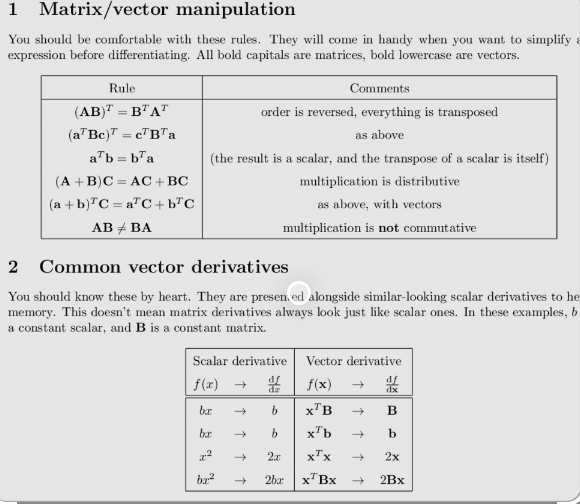
\includegraphics[scale=1]{vector calc.png}

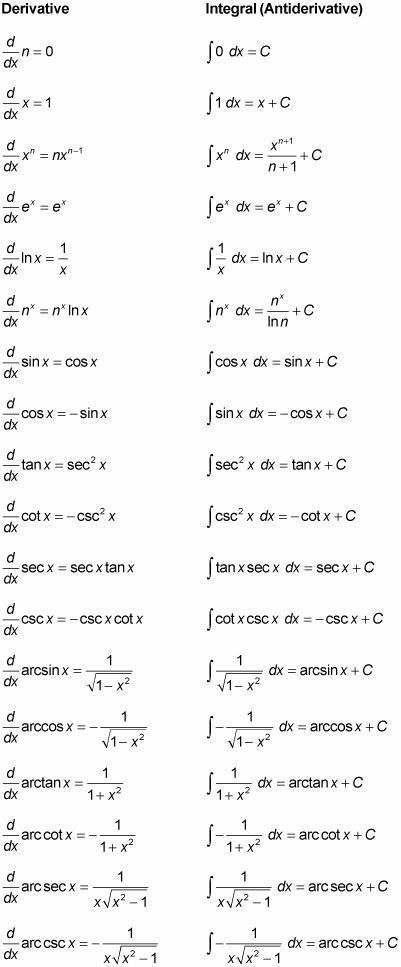
\includegraphics[scale=.6]{diff rom.jpg}

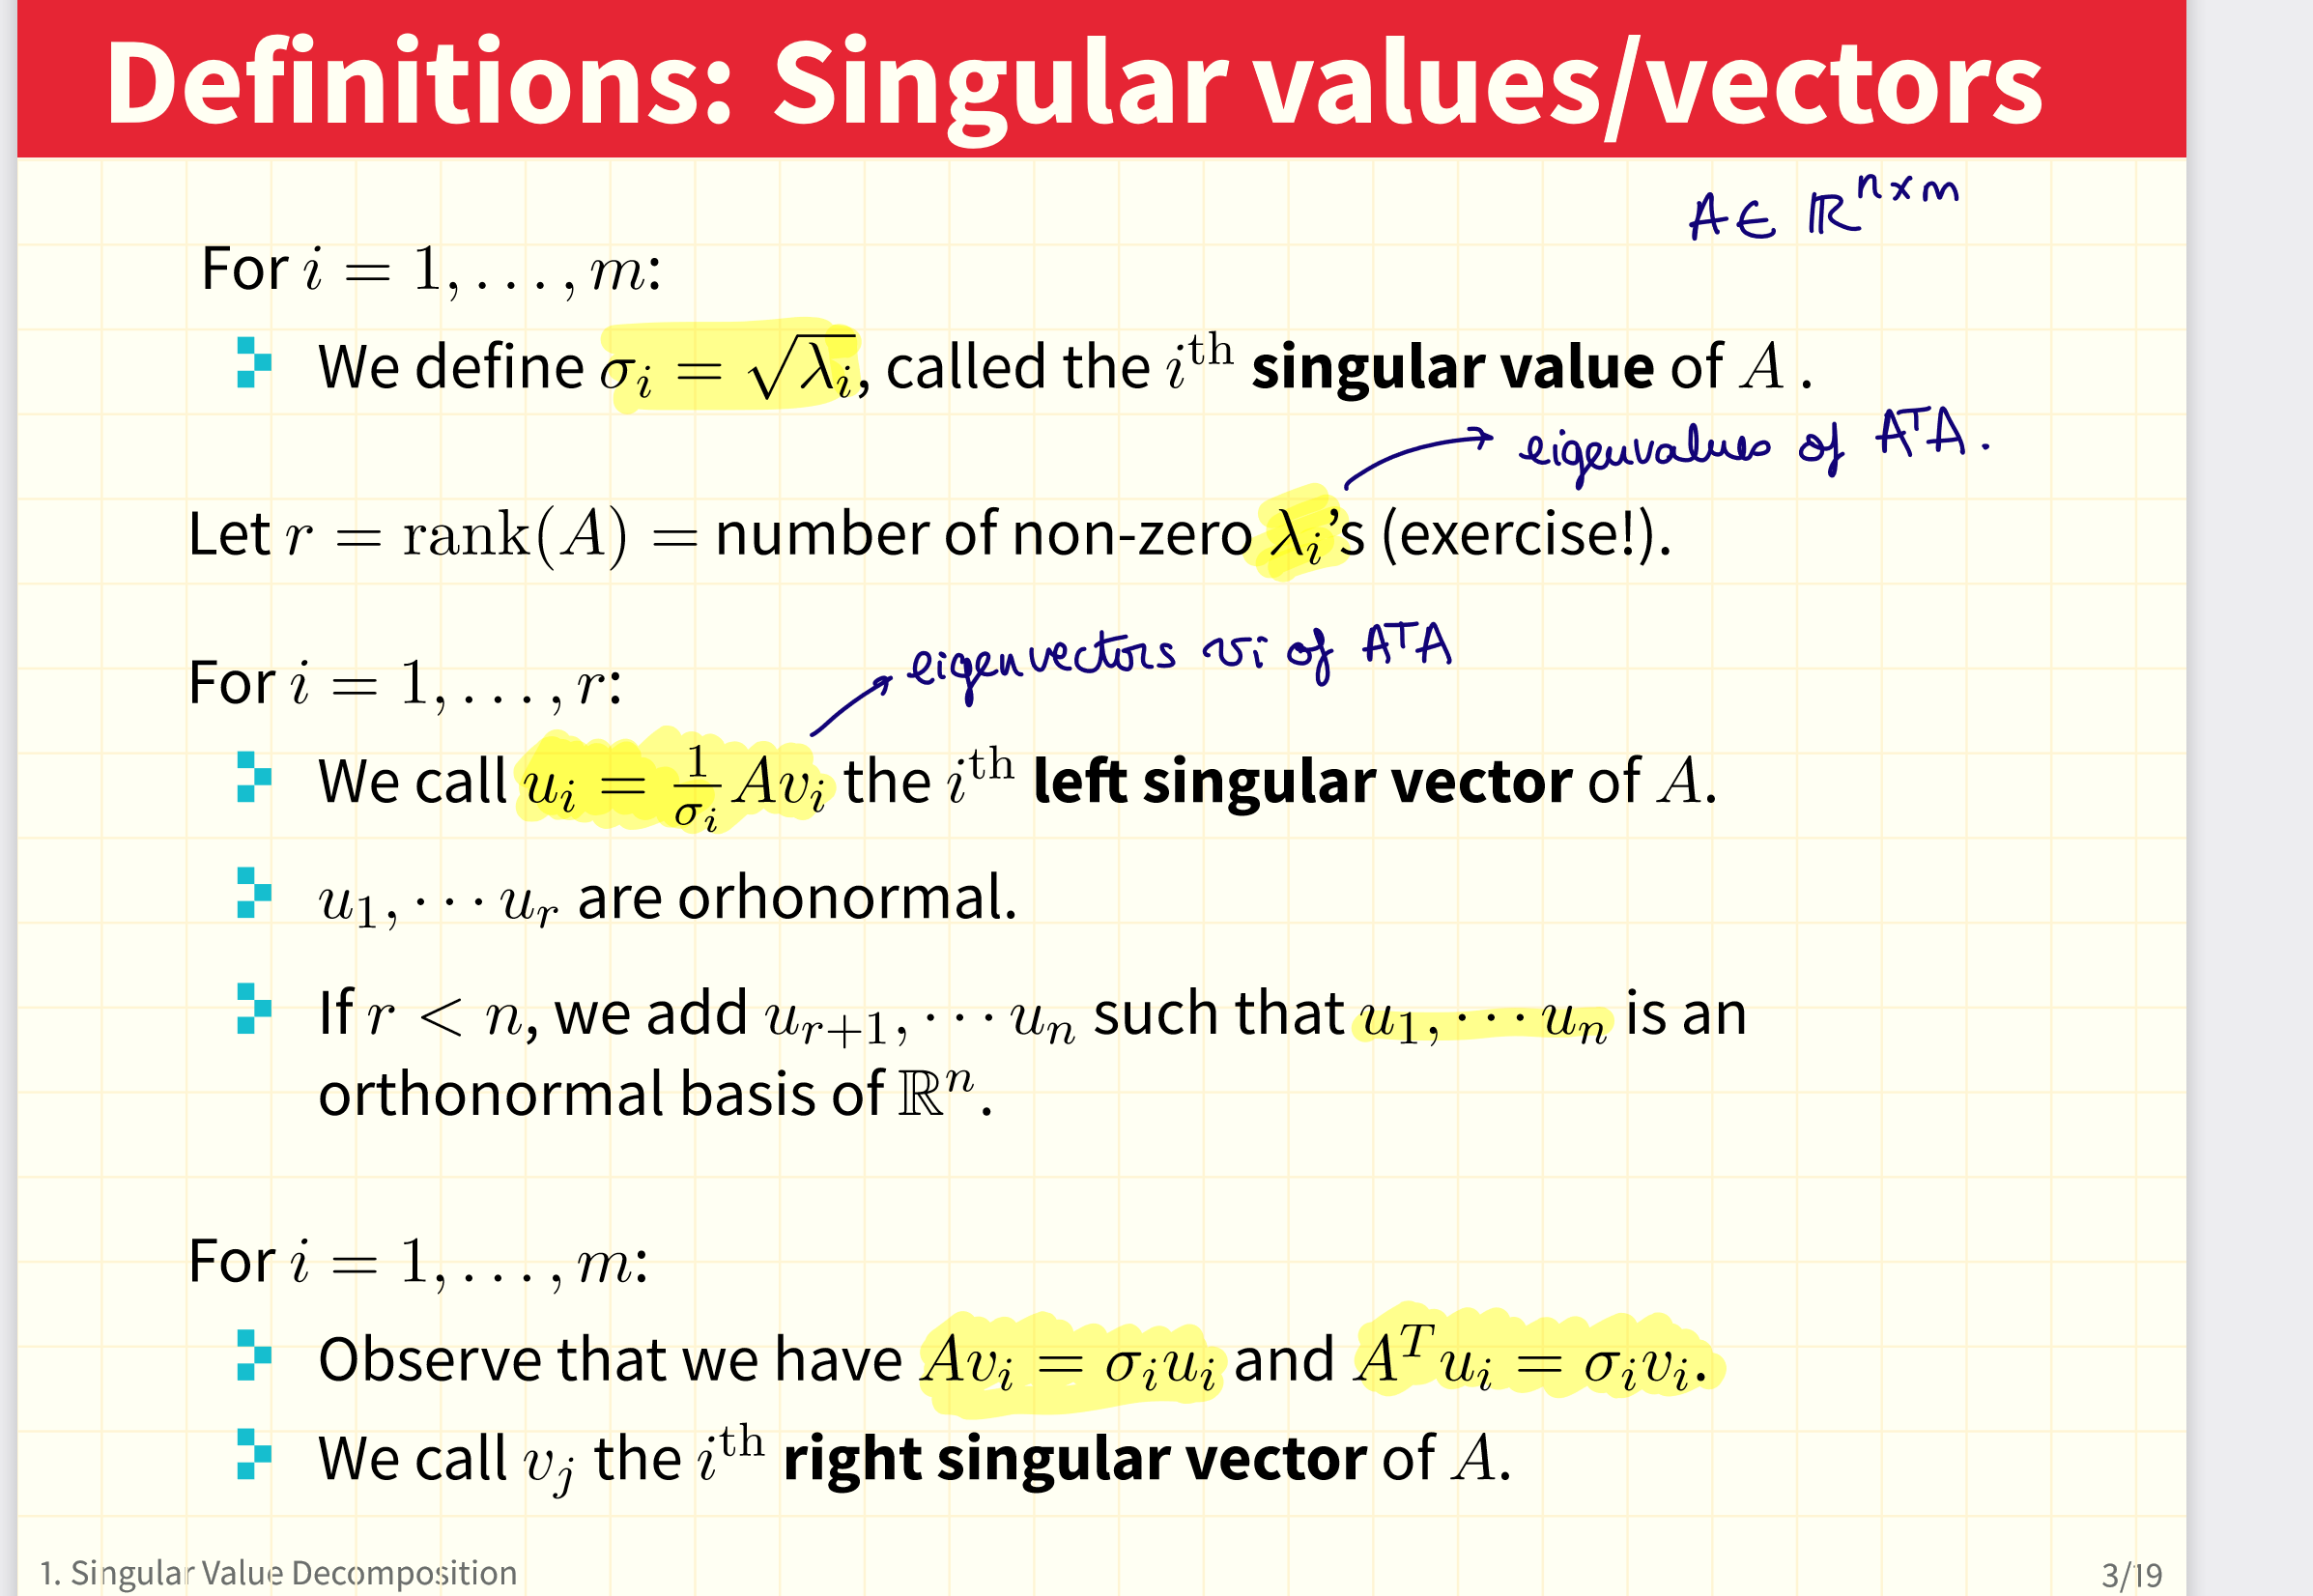
\includegraphics[scale=.5]{singular vectors.png}

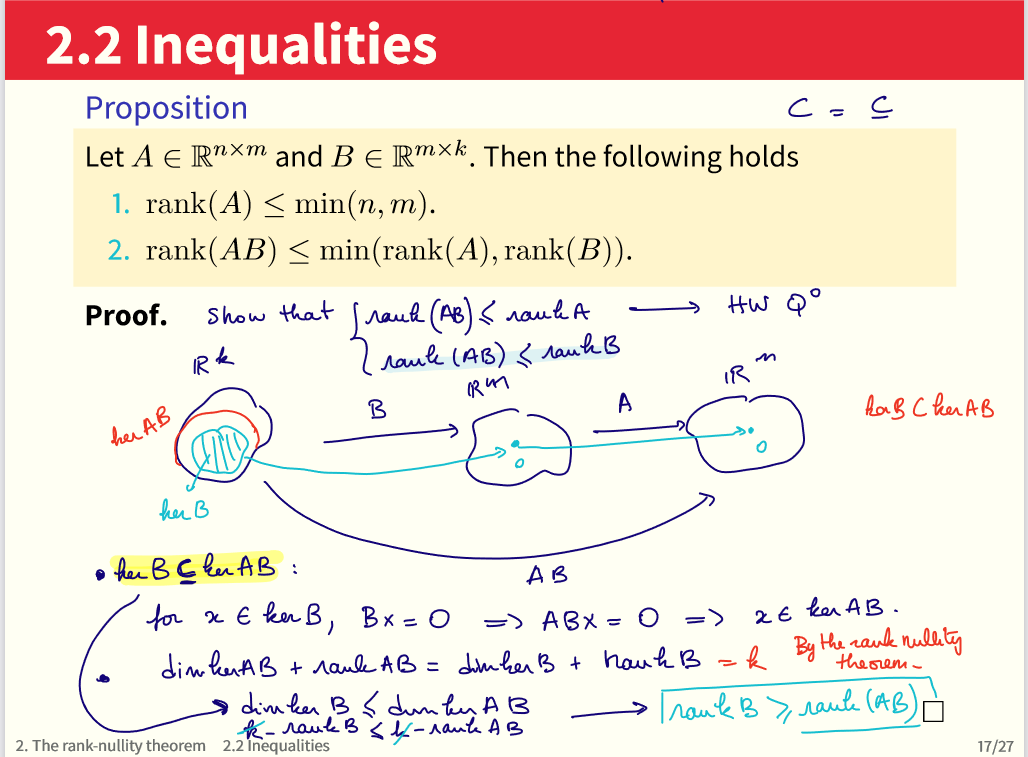
\includegraphics[scale=.6]{rank nul.png}

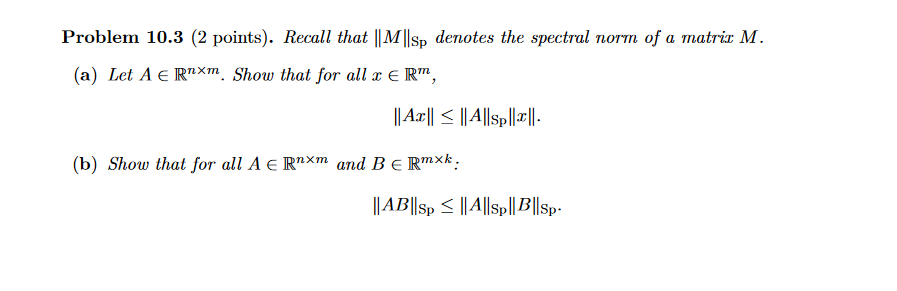
\includegraphics[scale=.85]{spectral norm q.png}

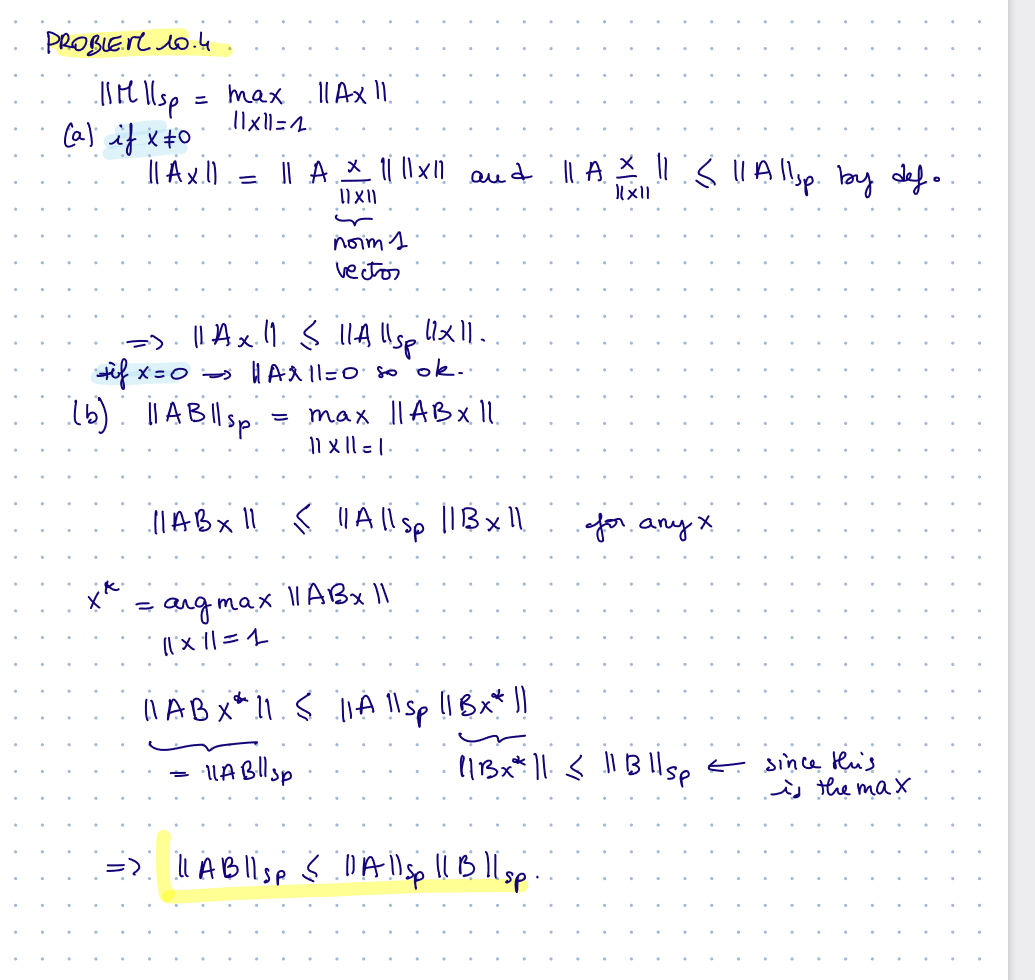
\includegraphics[scale=.55]{spectral norm proof.png}

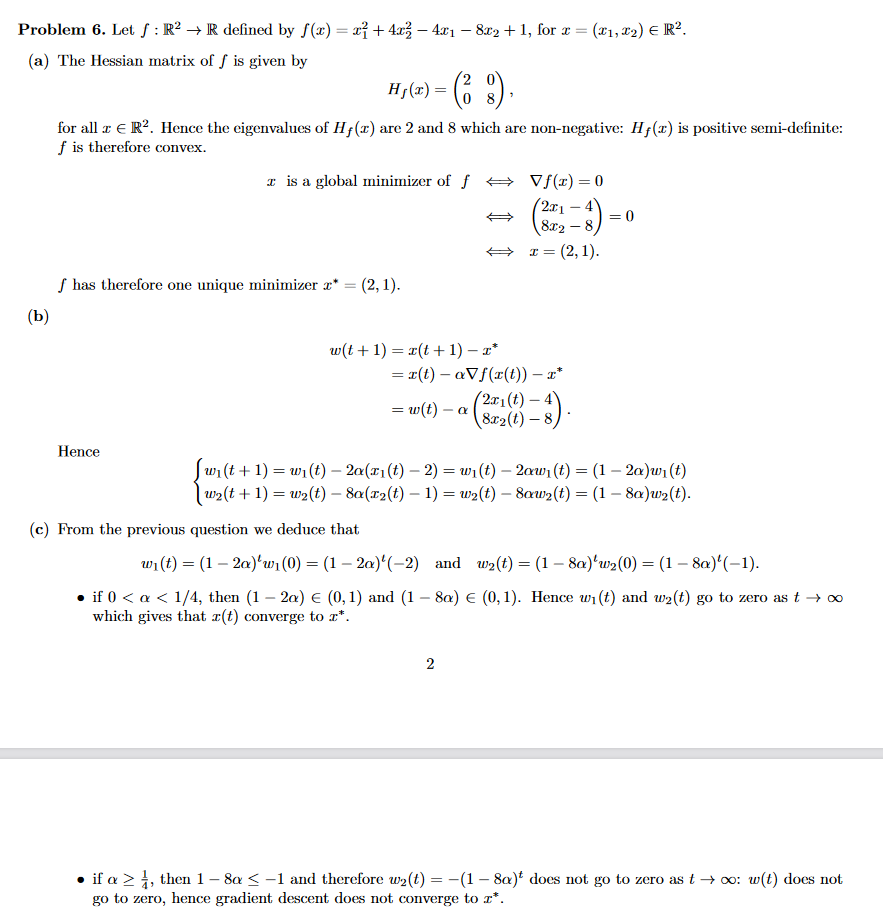
\includegraphics[scale=.7]{2019 final q 6.png}


\end{document}
